\section{Methodology}
\label{sec:method}

\subsection{Overall pipeline}
\label{sec:method-overall}

Figure~\ref{fig:pipeline} summarizes the parser. Word and POS tag embeddings are summed with a frozen pretrained word vector and concatenated, fed to a contextual encoder, projected by two MLPs into head-role and dependent-role vectors, and scored by a biaffine arc/relation module. Inference uses Chu--Liu--Edmonds MST decoding on the arc score matrix. The encoder slot accepts three implementations selected at construction time: \texttt{lstm} (the original three-layer BiLSTM), \texttt{transformer} (a parameter-matched SDPA Transformer), and \texttt{transformer\_large} (a deeper SDPA Transformer with modern training tricks). Every other component is shared across runs.

\begin{figure}[t]
  \centering
  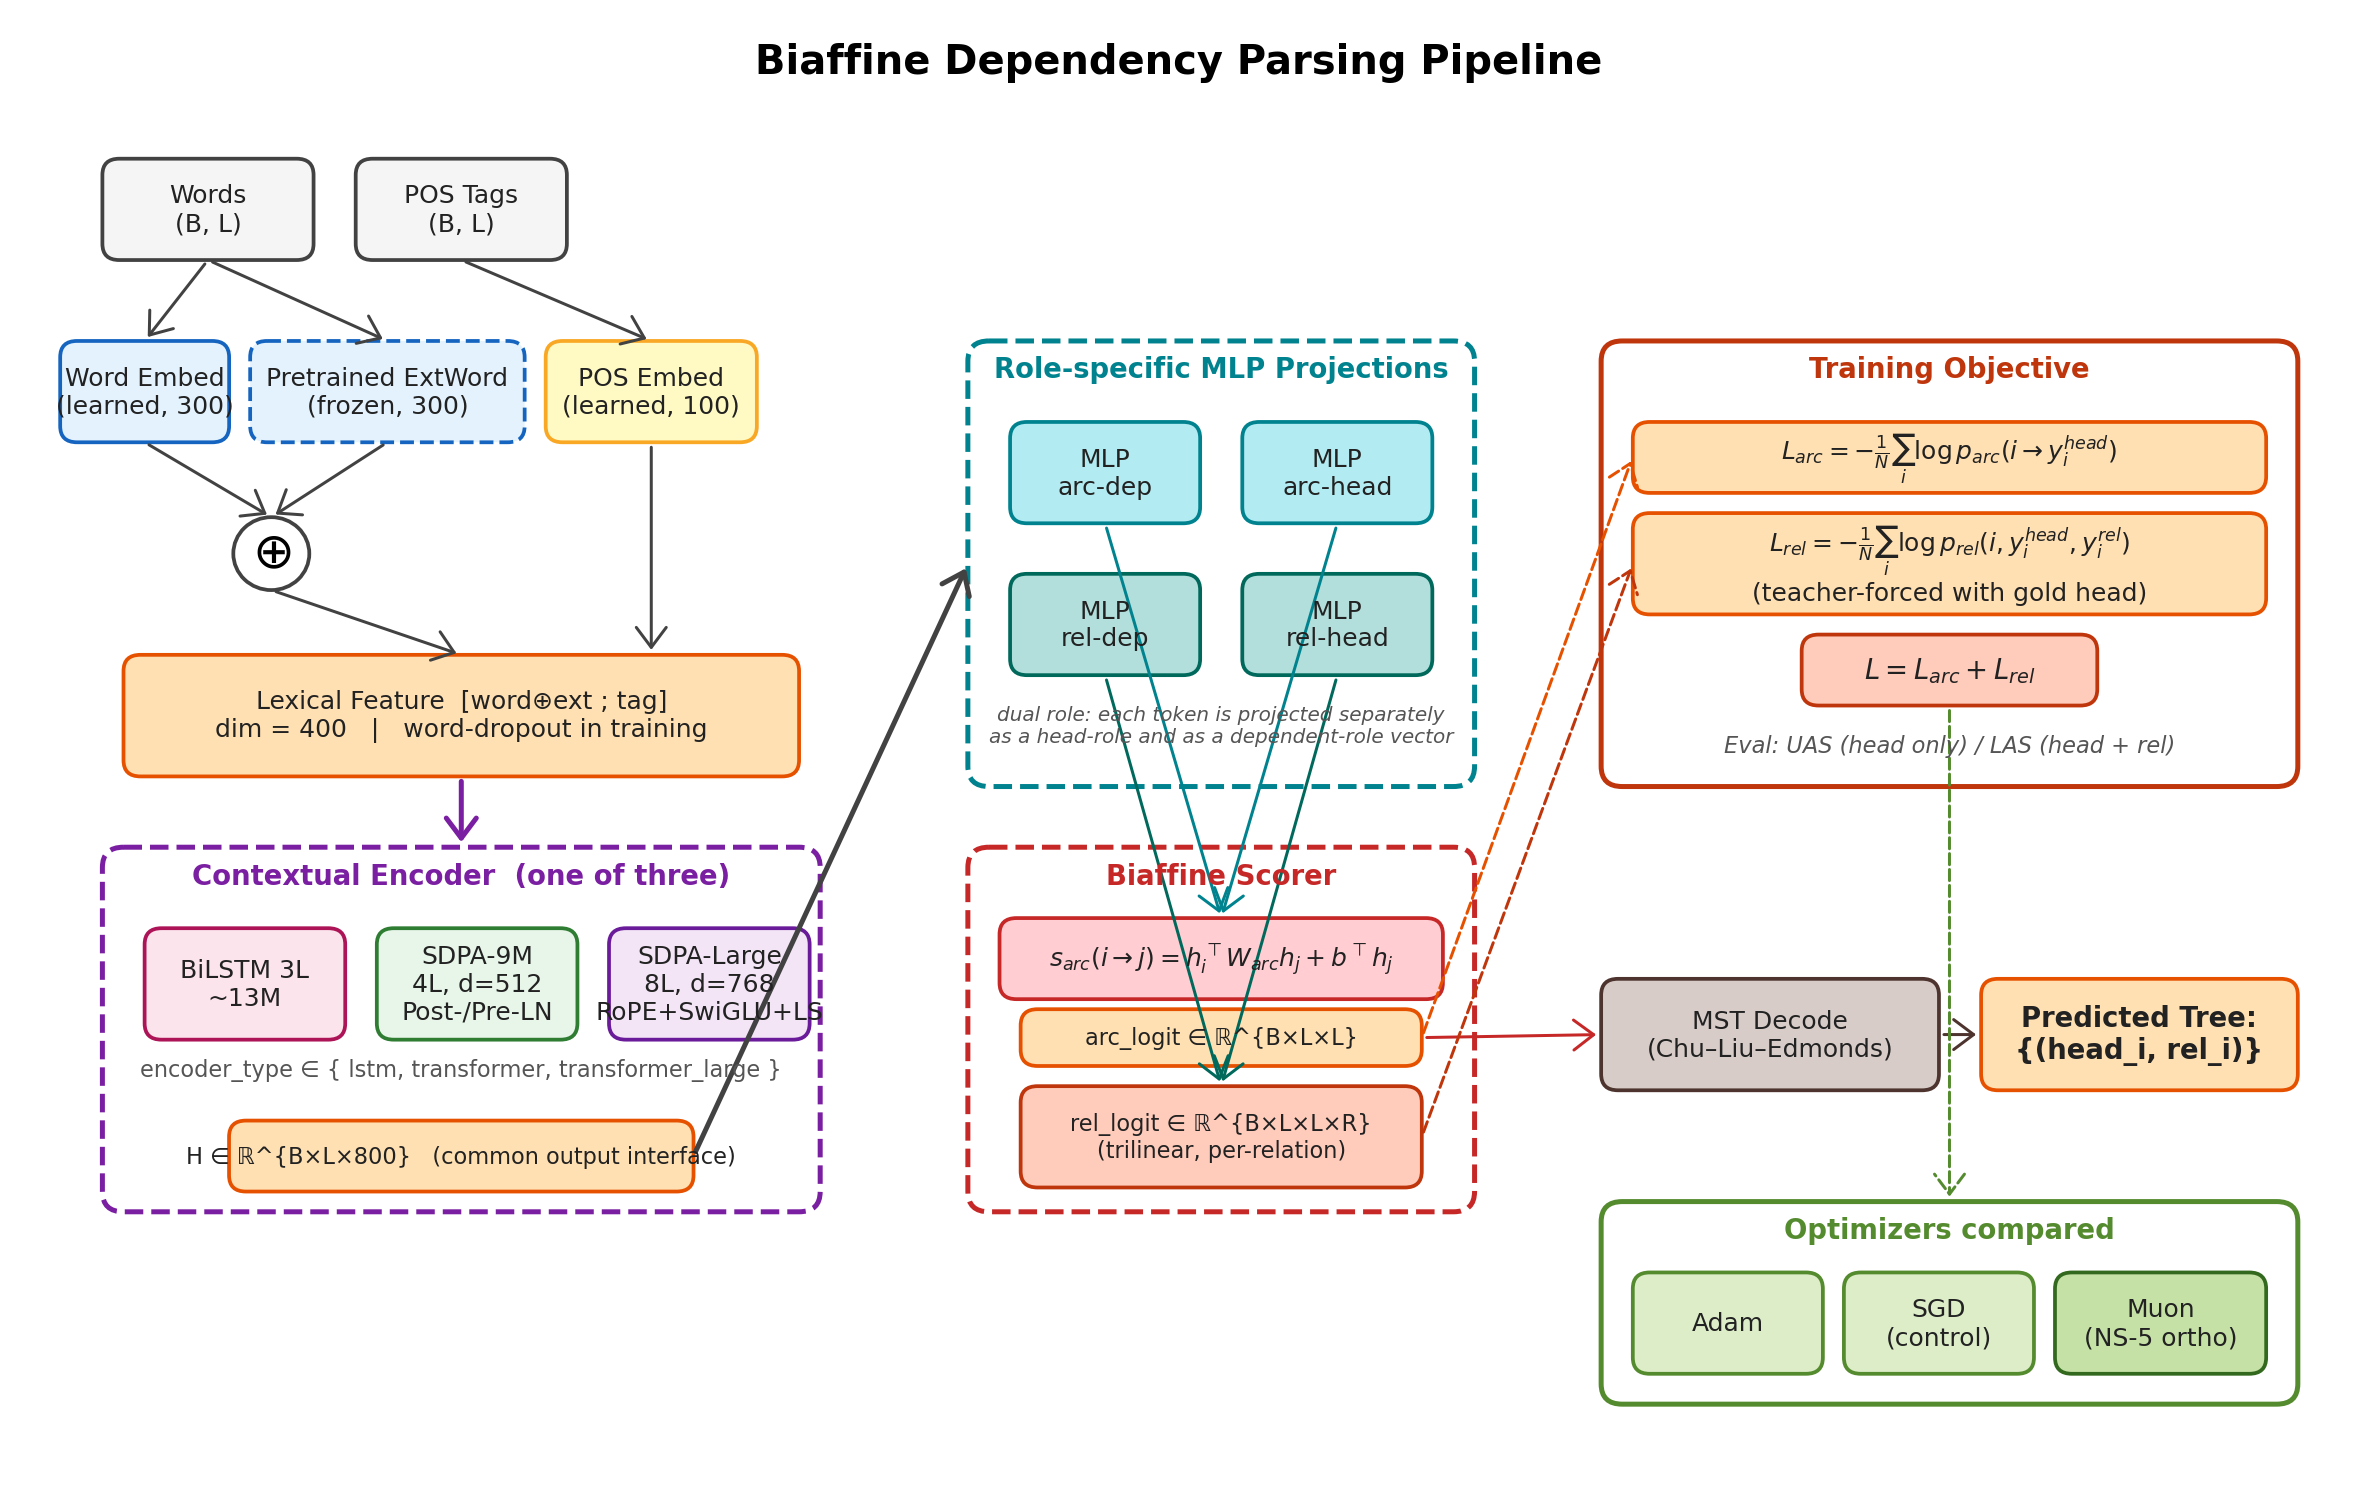
\includegraphics[width=0.95\linewidth]{figures/pipeline.png}
  \caption{Biaffine dependency parsing pipeline used throughout the paper. Three encoder slots (BiLSTM, SDPA-9M, SDPA-Large) plug into the same embedding stack on the left and the same biaffine--MST head on the right; only the encoder and the optimizer change across our fourteen runs. Key take-away: every accuracy difference reported is attributable to the encoder slot or the optimizer slot, not to the rest of the harness.}
  \label{fig:pipeline}
\end{figure}

\subsection{Embedding layer}
\label{sec:method-embedding}

A learned word embedding $\bW^{\text{word}}$ is summed with a frozen pretrained embedding $\bW^{\text{ext}}$ from the Chinese-Word-Vectors collection \citep{li2018cwv}; a separate learned 100-dim POS embedding is concatenated. Following \citet{dozat2017biaffine} we apply \emph{word dropout}, which zeros entire token embeddings independently with probability $p$, in addition to standard activation dropout.

\subsection{Encoder variants}
\label{sec:method-encoder}

Three encoders plug into the same interface, all producing $\bH\in\mathbb{R}^{L\times 800}$ for the downstream MLPs.

\paragraph{BiLSTM.} Three-layer bidirectional LSTM with 400 hidden units per direction, orthonormal recurrent initialization \citep{dozat2017biaffine}, and variational dropout (the same dropout mask reused across timesteps within a sequence). Implemented on top of \texttt{nn.LSTMCell}. About 13M parameters.

\paragraph{SDPA-9M.} Four-layer Transformer with $d_{\text{model}}=512$, $h=8$ heads, $d_{\text{ff}}=1024$, sinusoidal positional encoding. Parameter count is matched to the BiLSTM (about 9M) so that the encoder-family comparison is not contaminated by capacity. Padding is handled by an explicit \texttt{key\_padding\_mask}, and padding positions are zeroed before the output projection so that the bilinear scorer is not fed attention-leaked noise. We run two layout variants of this encoder: \emph{post-norm} (Vaswani-style $\bX'=\text{LN}(\bX+\text{Sub}(\bX))$) and \emph{pre-norm} ($\bX'=\bX+\text{Sub}(\text{LN}(\bX))$, \citealt{xiong2020lnorder}).

\paragraph{SDPA-Large.} Eight-layer Transformer with $d_{\text{model}}=768$, $h=12$, $d_{\text{ff}}=3072$ (about 76M parameters), combining four modern training tricks: pre-norm residuals, RoPE for query/key rotation \citep{su2021roformer}, SwiGLU feed-forward blocks \citep{shazeer2020glu}, and per-channel LayerScale initialised at $10^{-4}$ \citep{touvron2021cait}. We refer to this as \emph{SDPA-Large} throughout the rest of the paper, not as a SOTA configuration: it is the largest encoder we trained, but it does not achieve state-of-the-art on this treebank.

\subsection{Attention layer}
\label{sec:method-attention}

We use PyTorch's \texttt{F.scaled\_dot\_product\_attention} kernel, which dispatches at runtime to a FlashAttention-style implementation when eligible. RoPE is applied immediately before the kernel via the rotation in Equation~(\ref{eq:rope}). The bilinear attention used inside the biaffine head is a separate object; we describe it in Section~\ref{sec:theory}.

\subsection{Optimizers}
\label{sec:method-optimizer}

We compare three optimizers:
\begin{itemize}[leftmargin=*, itemsep=2pt]
  \item \textbf{Adam}, $\beta_1{=}0.9$, $\beta_2{=}0.9$, $\epsilon{=}10^{-12}$, following \citet{dozat2017biaffine}; the unusual small $\beta_2$ is suited to the BiLSTM and we keep it for backward compatibility.
  \item \textbf{SGD} with $\eta{=}10^{-2}$, no momentum, no schedule. Included as a negative control.
  \item \textbf{Muon} \citep{jordan2024muon}: each 2D non-embedding weight is updated via Newton--Schulz orthogonalization of its momentum buffer with per-tensor scale $\max(1,\sqrt{m/n})$. All other parameters (1D, embeddings) fall back to AdamW. Default $\eta_{\text{Muon}}{=}0.02$, $\eta_{\text{AdamW}}{=}3{\times}10^{-4}$. We package the routing logic in a wrapper so the standard \texttt{step}/\texttt{zero\_grad}/\texttt{state\_dict} interface remains intact.
\end{itemize}
